\documentclass[12pt]{article}
\usepackage[margin=1.2in]{geometry}
\usepackage[all]{nowidow}
\usepackage[hyperfigures=true, hidelinks, pdfhighlight=/N]{hyperref}
\usepackage[separate-uncertainty=true,group-digits=false]{siunitx}
\usepackage{graphicx,amsmath,physics,tabto,float,amssymb,pgfplots,verbatim,tcolorbox}
\usepackage{listings,xcolor,subfig,keyval2e,caption,import}
\numberwithin{equation}{section}
\numberwithin{figure}{section}
\numberwithin{table}{section}
\definecolor{stringcolor}{HTML}{C792EA}
\definecolor{codeblue}{HTML}{2162DB}
\definecolor{commentcolor}{HTML}{4A6E46}
\lstdefinestyle{appendix}{
    basicstyle=\ttfamily\footnotesize,commentstyle=\color{commentcolor},keywordstyle=\color{codeblue},
    stringstyle=\color{stringcolor},showstringspaces=false,numbers=left,upquote=true,captionpos=t,
    abovecaptionskip=12pt,belowcaptionskip=12pt,language=Python,breaklines=true,frame=single}
\lstdefinestyle{inline}{
    basicstyle=\ttfamily\footnotesize,commentstyle=\color{commentcolor},keywordstyle=\color{codeblue},
    stringstyle=\color{stringcolor},showstringspaces=false,numbers=left,upquote=true,frame=tb,
    captionpos=b,language=Python}
\renewcommand{\lstlistingname}{Appendix}
\pgfplotsset{compat=1.17}

\title{Hall Effect}
\author{KDSMIL001 \; PHY2004W PHyLAB 2}
\date{\textbf{17 November 2020}}

\begin{document}
    \begin{titlepage}
        \maketitle
        \center
        \tableofcontents
    \end{titlepage}
    
    \section{Introduction}\label{sec:Introduction}
    The Hall Effect is a well known effect that tells us a lot about the way that electric 
    charge conducts in materials. We will use it to determine some properties of the material 
    we're using, which is the p-type semiconductor germanium. 

    \section{Theory}\label{sec:Theory}
    If we have a block of material that conducts electricity and we put some current through it 
    there will be some kind of charge carrier moving through the material. Depending on the 
    material this could be either electrons, which are negatively charged, or positively charged 
    ''holes". If the material in question is placed within a magnetic field these moving charges 
    will feel a force in a direction perpendicular to their movement, dictated by 
    \begin{equation}
        \vec{F}=q\vec v\times\vec B
        \label{eqn:Lorentz Force}
    \end{equation}
    Because this force is perpendicular to the direction of movement of the charge carriers, we 
    will see some charge build-up on one side of the material, and a lack of charge on the other. 
    This means we can measure the voltage drop across the sides of the material. This voltage 
    is governed by the equation
    \begin{equation}
        V_\perp=R_H I_S B/c
        \label{eqn:V Perp}
    \end{equation}
    where $B$ is the strength of the magnetic field, $I_S$ is the applied current, and 
    $R_H\equiv \frac{1}{nq}$ is known as the Hall coefficient, with $n$ being the number of 
    charge carriers in the material and $q$ being the amount of charge each carrier can carry. 
    \newline
    We can also measure the voltage drop across the length of the material, in the direction the 
    current is flowing. That voltage is given by 
    \begin{equation}
        V_\parallel=\frac{I_s b}{\sigma a c}
        \label{eqn:V parallel}
    \end{equation}
    where $\sigma$ is the electrical conductivity of the material. $a$, $b$, and $c$ as well 
    as the general set-up of the material is shown below.
    \begin{figure}[H]
        \begin{center}
            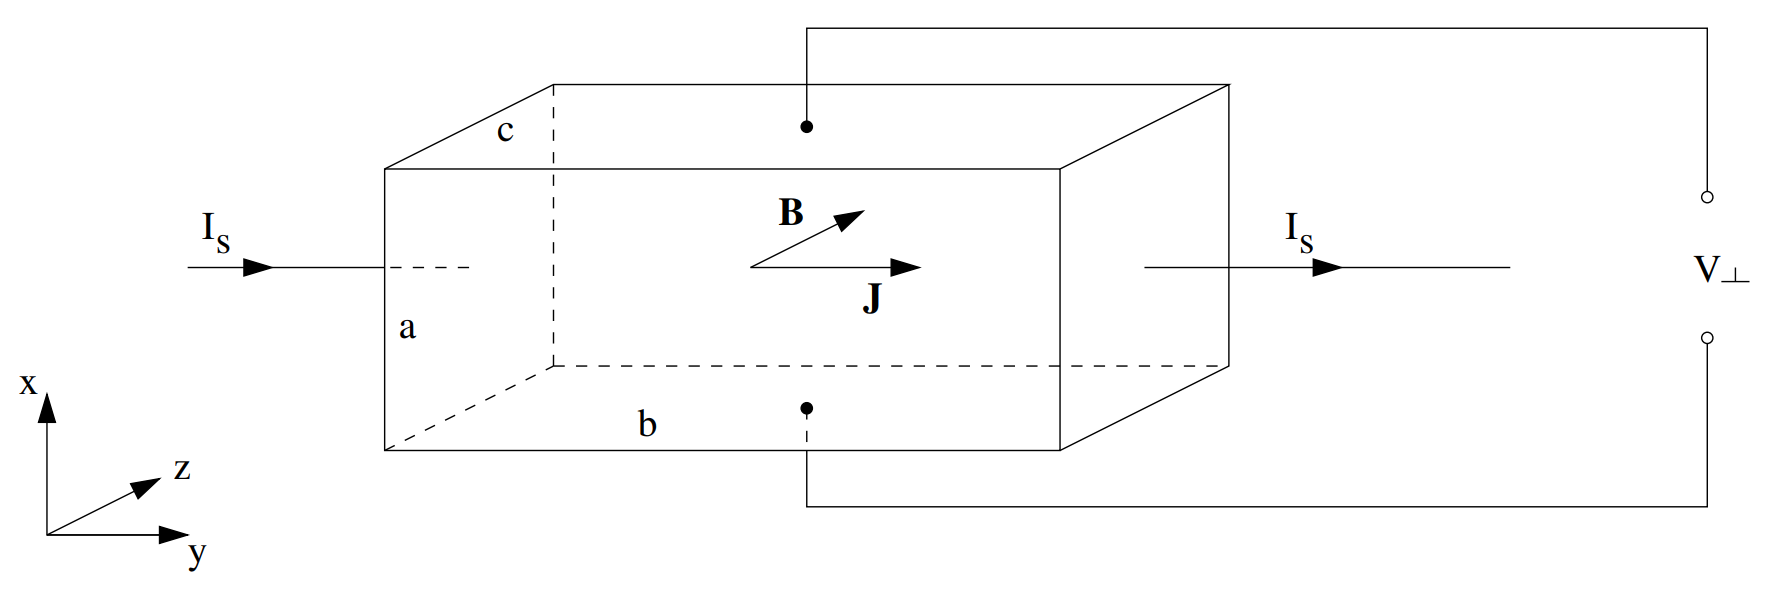
\includegraphics[width=.65\textwidth]{MaterialSetup.png}
            \label{fig:MaterialSetup}
        \end{center}
    \end{figure}
    By knowing all the other values, we can find values for $R_H$ and $\sigma$. \newline
    Since we are using germanium, which is a semiconductor, the definition for $R_H$ is slightly 
    different, it even depends on what type of charge carrier the semiconductor has. For p-type 
    semiconductors, which germanium is, the Hall coefficient is given by 
    \begin{equation}
        R_H=\frac{1.4}{n e}
        \label{eqn:Hall Coefficient p-type}
    \end{equation}
    with $e$ being the charge on an electron, $e=\SI{1.60217662e-19}{\coulomb}$. \newline
    \newline
    Now all this theory is based on the idea that the material in question stays at the same 
    temperature, since in semiconductors both the number of charges and their mobility within the 
    material are dependent on temperature. The problem is that as we drive a current through the 
    germanium, it is going to heat up thanks to Joule heating. \autoref{eqn:V Perp} and 
    \autoref{eqn:V parallel} are both linear, but since we expect values to change depending on 
    the temperature of the material, we can expect to see some deviation from linearity. 
    
    \section{Apparatus}\label{sec:Apparatus}
    \begin{itemize}
        \item DC power supply.
        \item Offset potentiometer.
        \item A 500 $\si[]{\ohm}$ resistor. 
        \item Multimeter set to 200 mA scale to measure the current through the material.
        \item Multimeter set to 200 mV scale to measure the Hall voltage. 
        \item Multimeter set to 20 V scale to measure the voltage along the sample. 
        (All multimeters have $\pm 1\%$ error.)
        \item A piece of germanium. (See \autoref{fig:GermaniumDimensions}.)
    \end{itemize}
    \begin{figure}[H]
        \begin{center}
            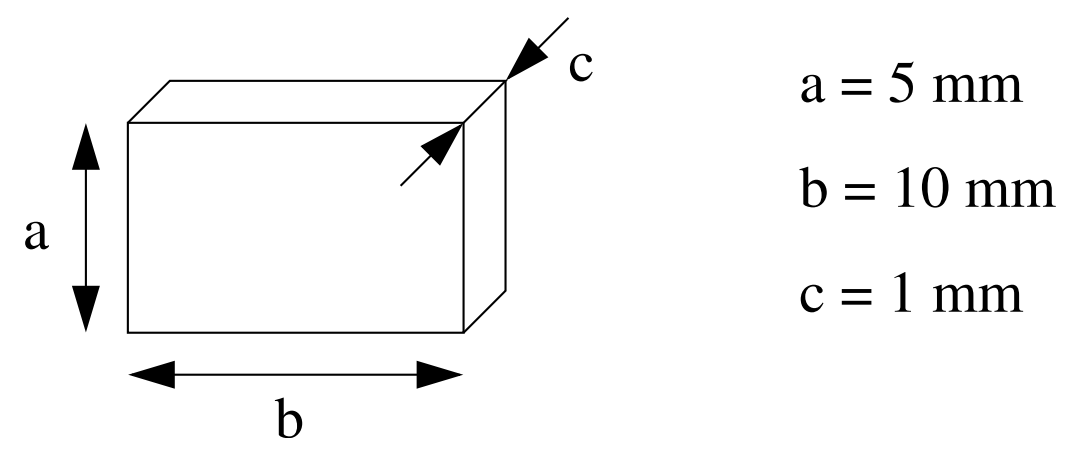
\includegraphics[width=.4\textwidth]{GermaniumDimensions.png}
            \caption{The dimensions of the sample of germanium used}
            \label{fig:GermaniumDimensions}
        \end{center}
    \end{figure}
    \begin{figure}[H]
        \begin{center}
            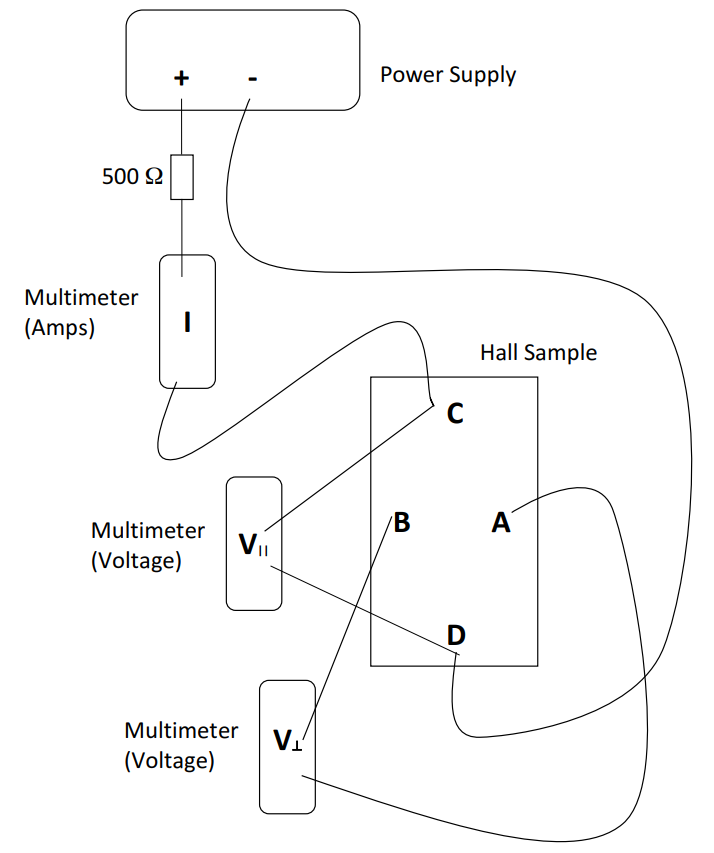
\includegraphics[width=.65\textwidth]{CircuitDiagram.png}
            \caption{The set-up of the circuit}
            \label{fig:CircuitDiagram}
        \end{center}
    \end{figure}
    The potentiometer is used so we can adjust things to make sure that the Hall voltage is 
    0 when there is no magnetic field present, as a sort of calibration. 

    \section{Method}\label{sec:Method}
    The order of the steps taken is very important. They are as follows:
    \begin{enumerate}
        \item We connected the circuit as shown in \autoref{fig:CircuitDiagram}. It is 
        important that the current through the sample does not exceed 50 mA so the 500 
        $\si[]{\ohm}$ resistor must be in place before switching the power supply on. 
        \item Before switching the power supply on, we set the current controls to their 
        maximum and the voltage controls to their minimum, then turned the power supply on. 
        \item We then adjusted the voltage to 22 V on the power supply display, making sure 
        that the current measured by our multimeter doesn't exceed 40 mA.
        \item We then set the current in the sample to about 38 mA with no magnetic field 
        near to the sample, varying our potentiometer to obtain a Hall voltage of 0 V. 
        \item We then measured the Hall voltage, $v_\perp$, and the voltage along the sample, 
        $V_\parallel$, as a function of the current $I$ over the range 0 to 40 mA. We made sure 
        not to exceed 22 V on the power supply display. We call this the forward data. 
        \item We then left the circuit running at 40 mA for 10 minutes, allowing the sample to 
        heat up, and then performed the same measurements, this time going backwards. 
    \end{enumerate}
    Some important things to note: We measured the temperature of the sample before we started 
    and found it to be 25.4 C, as well as after the 10 minutes at 40 mA, finding that 
    to be 31.3 C. This change is as a result of the Joule heating mentioned earlier. 
    
    \section{Results}\label{sec:Results}
    \begin{figure}[H]
        \begin{center}
           \scalebox{.7}{\subimport{Data}{ForwardParallel.pgf}}
           \caption{$V_\parallel$ plotted against $I_S$ for the data collected going forward.}
           \label{fig:ForwardParallel}
        \end{center}
    \end{figure}
    \begin{figure}[H]
        \begin{center}
           \scalebox{.7}{\subimport{Data}{ForwardPerp.pgf}}
           \caption{$V_\perp$ plotted against $I_S$ for the data collected going forward.}
           \label{fig:ForwardPerp}
        \end{center}
    \end{figure}
    \begin{figure}[H]
        \begin{center}
           \scalebox{.7}{\subimport{Data}{BackwardParallel.pgf}}
           \caption{$V_\parallel$ plotted against $I_S$ for the data collected going backwards.}
           \label{fig:BackwardParallel}
        \end{center}
    \end{figure}
    \begin{figure}[H]
        \begin{center}
           \scalebox{.7}{\subimport{Data}{BackwardPerp.pgf}}
           \caption{$V_\perp$ plotted against $I_S$ for the data collected going backwards.}
           \label{fig:BackwardPerp}
        \end{center}
    \end{figure}
    As a check of linearity we have calculated $V_\perp/I_S$ and $V_\perp/V_\parallel$ for each 
    set of data and below are the approximate means and variances of each set.
    \begin{table}[H]
        \centering
        \begin{tabular}{c|c|c}
             & Forward & Backwards \\
            \hline
            $V_\perp/I_S$ & & \\
            Mean & $1.488$ & $1.538$ \\
            Variance & $0.00338$ & $0.00503$ \\
            \hline
            $V_\perp/V_\parallel$ & & \\
            Mean & $0.0129$ & $0.0132$ \\
            Variance & $\num{8.494e-8}$ & $\num{1.149e-7}$ \\
        \end{tabular}
        \caption{Means and Variances for $V_\perp/I_S$ and $V_\perp/V_\parallel$ for both the 
        forward and backwards data sets.}
        \label{tbl:MeanVariance}
    \end{table}
    We also want to find values for $R_H$, $\sigma$, and $n$. To do this we use 
    \autoref{eqn:V Perp}, \autoref{eqn:V parallel}, and \autoref{eqn:Hall Coefficient p-type}. 
    We could look at these equations and see that, if the data was linear we could find the 
    gradients and get very accurate estimations for these values, but our data isn't linear, 
    so we must select the "best values" and just work with that. We have decided that the 
    best values would be those measured at the beginning of the experiment when the germanium 
    hadn't heated up that much. So that would be the first non-zero values in the forward data.
    \newline So we have
    \begin{align*}
        R_H&=\frac{V_\perp c}{I_s B}\\
        &=\frac{0.0028\cdot0.001}{0.002\cdot0.125}\\
        &=0.0112\\
        u(R_H)&=R_H\sqrt{\left(\frac{u(V_\perp)}{V_\perp}\right)^2+\left(\frac{u(I_S)}{I_S}\right)^2+\left(\frac{u(B)}{B}\right)^2}\\
        u(V_\perp)&=\sqrt{\left(\frac{\num{0.1e-3}}{2\sqrt3}\right)^2+(1\%\cdot \num{100e-3})^2}\\
        &=\SI{1e-3}{\volt}\\
        u(I_S)&=\sqrt{\left(\frac{\num{0.1e-3}}{2\sqrt3}\right)^2+(1\%\cdot \num{100e-3})^2}\\
        &=\SI{1e-3}{\ampere}\\
        u(B)&=0.005\\
        \implies u(R_H)&=\num{5.632113635e-3}
    \end{align*}
    \begin{align*}
        \sigma&=\frac{I_s b}{acV_\parallel}\\
        &=\frac{0.002\cdot0.01}{0.005\cdot0.001\cdot0.22}\\
        &=18.1818\overline{18}\\
        u(\sigma)&=\sigma\sqrt{\left(\frac{u(I_S)}{I_S}\right)^2+\left(\frac{u(V_\parallel)}{V_\parallel}\right)^2}\\
        u(V_\parallel)&=\sqrt{\left(\frac{0.01}{2\sqrt3}\right)^2+(1\%\cdot 10)^2}\\
        &=\SI{0.1001}{\volt}\\
        \implies u(\sigma)&=12.28600723
    \end{align*}
    \begin{align*}
        n&=\frac{1.4}{R_H e}\\
        &=\frac{1.4}{0.0112\cdot\num{1.60217662e-19}}\\
        &=\num{7.801886411e20}\\
        u(n)&=\frac{1.4}{e}\cdot u(1/R_H)\\
        &=\num{3.92331e21}
    \end{align*}
    We can also find $\mu$, the mobility of the charge carriers in the superconductor. It is 
    given by 
    \begin{align*}
        \mu&=\frac{\sigma}{ne}\\
        &=\frac{18.181818}{\num{7.801886411e20}\cdot\num{1.60217662e-19}}\\
        &=0.14545\overline{45}\\
        u(\mu)&=\mu\sqrt{\left(\frac{u(\sigma)}{\sigma}\right)^2+\left(\frac{u(n)}{n}\right)^2}\\
        &=0.739269
    \end{align*}
    So we have
    \begin{table}[H]
        \centering
        \begin{tabular}{c|c}
            $R_H$ & $\SI{0.0112\pm0.0056}{\metre^3 \coulomb^{-1}}$ \\
            $\sigma$ & $\SI{18\pm12}{\siemens\metre^{-1}}$\\
            $n$ & $\num{0.78\pm3.9e21}$\\
            $\mu$ & $\SI{0.14\pm0.74}{\metre^2\volt^{-1}\second^{-1}}$
        \end{tabular}
        \caption{Values for room temperature germanium}
        \label{tbl:Room Temp}
    \end{table}
    \textbf{Exercises:}
    Regarding the change in conductivity of the sample with respect to temperature, we can 
    calculate the values calculated above from the reading taken after 10 minutes at 40 mA:
    \begin{enumerate}
        \item 
        \begin{align*}
            \sigma&=\frac{I_s b}{acV_\parallel}\\
            &=\frac{0.040\cdot0.01}{0.005\cdot0.001\cdot4.81}\\
            &=16.63201663\\
            u(\sigma)&=12.28600723
        \end{align*}
        \item 
        \begin{align*}
            R_H&=\frac{V_\perp c}{I_s B}\\
            &=\frac{0.0661\cdot0.001}{0.04\cdot0.125}\\
            &=0.01322\\
            u(R_H)&=\num{5.632113635e-3}\\
            n&=\frac{1.4}{R_H e}\\
            &=\frac{1.4}{0.01322\cdot\num{1.60217662e-19}}\\
            &=\num{6.60976761e20}\\
            u(n)&=\num{2.815957812e21}
        \end{align*}
        \item 
        \begin{align*}
            \mu&=\frac{\sigma}{ne}\\
            &=\frac{16.63201663}{\num{6.60976761e20}\cdot\num{1.60217662e-19}}\\
            &=0.157053757\\
            u(\mu)&=0.679079252
        \end{align*}
    \end{enumerate}
    We have 
    \begin{table}[H]
        \centering
        \begin{tabular}{c|c}
            $R_H$ & $\SI{0.0132\pm0.0056}{\metre^3 \coulomb^{-1}}$ \\
            $\sigma$ & $\SI{16\pm12}{\siemens\metre^{-1}}$\\
            $n$ & $\num{0.66\pm3.9e21}$\\
            $\mu$ & $\SI{0.15\pm0.68}{\metre^2\volt^{-1}\second^{-1}}$
        \end{tabular}
        \caption{Values for higher than room temperature germanium}
        \label{tbl:High Temp}
    \end{table}

    \section{Discussion}\label{sec:DiscussionRecommendations}
    Looking at the figures in \autoref{sec:Results}, we see that if we take a gradient from the 
    first two points and extend that line along the whole data set, we see that the data 
    deviates from linearity without exception. It deviates the most for the Hall voltage, which 
    makes sense as the values of the Hall voltage are much smaller than those for $V_\parallel$. 
    The backwards data also seems to be slightly more nonlinear than the forwards data. We are not 
    entirely sure why this is, but it might be that after the 10 minutes at 40 mA, the germanium 
    reached its peak temperature and then as the current decreased, it cooled down faster than 
    it heated up when taking the forwards data, but this is just speculation. \newline
    Regarding \autoref{tbl:MeanVariance}, we can see that while the variances are small, they are 
    still big enough relative to the mean values, which shows that there is some deviation in the 
    data sets, further indicating nonlinearity. 
    \textbf{Exercises:}
    \begin{enumerate}
        \item Our calculated value for $\sigma$ decreases as the temperature increases, but since 
        the uncertainty on both the room temperature and higher temperature values is so large, 
        it is hard to say for sure whether the conductivity increases or decreases with temperature. 
        What we expect is that the conductivity increases with temperature as more charge carriers 
        are released from the atoms of the material. Our results are inconclusive.

        \item Again we see the opposite of what we expect, since we should see more charge carriers, 
        but instead we see a decrease. Again, however, our results are inconclusive since the 
        uncertainty on both values is greater than the value itself.

        \item Lastly, we see a slight increase in mobility as temperature increases. Both values 
        agree within experimental uncertainty with the provided value of 
        $\SI{0.18}{\metre^2\volt^{-1}\second^{-1}}$, but not with the idea that mobility should 
        decrease with temperature. 
    \end{enumerate}
    We are not sure why we seem to observe the opposite of what we expect when increasing the 
    temperature of the sample. Perhaps the sample is not a pure semiconductor.

    \section{Conclusion}\label{sec:Conclusion}
    To conclude, we were able to find values for $R_H$, $\sigma$, $n$, and $\mu$ for a sample of 
    germanium, with varying levels of accuracy. When trying to investigate the effect of temperature 
    on these values, we observed the opposite to what we expect for a this material. We are not 
    sure why this has happened. 

\end{document}